\section{Pilot Experiment}\label{pilot}
In this section, we introduce the pilot experiment we conducted prior to the large scale experiment. In general pilot experiments are a method to test feasibility and provide experience-based guidelines for follow up experiments. 
\subsection{Introduction}
The pilot experiment was conducted in the facilities of Systems Neuroscience and Neurotechnology Unit, particularly the Mindscan Lab, located at the HTW Saar (Technikum). The main goal of this experiment was to gather an initial set of authentic data while also testing the functionality of our data transmission routine and familiarizing ourselves with hardware and software behavior under experiment conditions. \\
The measurement was performed in a closed off laboratory environment with controlled temperature and illumination. Physiological signals were recorded using the Empatica E4, which was placed on the wrist of the non-dominant hand, and a laptop, serving as Processing Unit, that was placed approximately 1.5 meters away from the subject position.
We measured 2 subjects in this pilot experiment. They were bachelor level male students, studying at the HTW Saar aged between 26 and 30 years.

\subsection{Objectives}
\begin{itemize}
\item Test the procedure and the experimental design
\item Identify problems and optimization possibilities
\item Estimation of time and resource requirements
\item Inspect data quality
\end{itemize}
\subsection{Setup}
The experimental setup can be divided into two major components. The first component, was responsible for data acquisition and was comprised of the Empatica E4 and the Processing Unit. Whereas the second, handled the presentation of the experimental paradigm using a second Notebook in combination with a monitor.
During the experiment the subject was positioned in a chair in front of a PC monitor. The recording site was surrounded by movable walls serving as visual cover. Directly behind the cover, and to the side of the recording site, a desk was placed to provide space for the Processing Unit, the operator, as well as any additional devices needed for the experiment. The distance between the E4, when worn by the subject, and the Processing Unit was approximately 1.5 meters.
%During the measurement the subjects were sitting in a chair, in an upright position, facing a monitor on the desk in front of them.
The room was calm and dimly lit, providing enough light to allow the participants to comfortably observe the paradigm on the monitor without any reflections, or being blinded by incident sun light. The temperature was regulated by an air conditioning system and kept at a constant level during the experiment to negate environmental influences.
\subsection{Procedure}
In preparation of the experiment all participants were given a step-by-step explanation of the experimental procedure, to make sure they were in a relaxed and comfortable mood. After, the subjects had given their consent, they were asked to remove any electronic devices from their person and take a seat in the chair. Then, they were instructed to put on the Empatica E4. If necessary an operator would assist them. Once they were finished, the operator inspected the placement of the wristband in regards to the general fit, and sensor-skin contact. Prior to the start of the paradigm the participants were again reminded to be as relaxed as possible, make themselves comfortable, and avoid extensive movement. During the experiment the subjects were required to sit in front of the monitor and observe the paradigm, which was displayed on it, for a period of 5 minutes. 
\subsection{Paradigm}
The paradigm that was used in the pilot experiment, was comprised of a single picture showing a simple black cross-hair on a white background. The paradigm was created with PsychoPy, which was running on a Notebook, connected to the monitor. 
\subsection{Problem Oriented}\label{po}
From the feedback we were given by the subjects, we were able to identify the following problems:
\begin{itemize}
\item The participants reported that the motive of the paradigm was causing them discomfort as the contrast between black and white was too extreme.
\item Both participants felt that the chair was not providing enough comfort due to missing armrests and height difference to the table. 
\end{itemize}
Further, we observed a slight offset in system time between the Processing Unit and the Notebook we used to run PsychoPy that could potentially raise issues in subsequent data analysis.

\subsection{Solution Oriented}
To address the aforementioned problems we altered the color scheme of our paradigm to provide a softer contrast (grey/white), exchanged the chair, and implemented a time synchronization routine in the experimental procedure.

\subsection{Results and Conclusion}
Because the results of our pilot experiment were overall positive we felt reassured to proceed to the main experiment with few alterations. We were able to successfully test the experimental procedure and the functionality of the setup. Further we were able to record quality data and gained valuable insight on the extent of the pre-processing needed to prepare the signals for feature extraction. We also gained a better understanding of the time-frame needed for the preparation, and the post-production of the experiment.

\newpage
\section{Main Experiment}
In this section we present the main experiment of this thesis, which was conducted subsequently to our pilot experiment.
\subsection{Introduction}
In the second experiment, we measured a larger group of subjects, aiming to collect a reasonable amount of data for machine learning. Therefore, the fundamental idea of this experiment was to elicit several emotional states in the participants by using a combination of cognitive tests and visual stimulation.  
Similar to the pilot experiment, we conducted prior, all measurements took place within the facilities of Systems Neuroscience and Neurotechnology Unit, particularly the Green Lab, located at the University Hospital Saarland, and the Mindscan Lab, located at the HTW Saar (Technikum). The sessions that took place at the Mindscan Lab, used the exact setup from the pilot measurement except for a few modifications to account for the problems that were identified in \ref{po}. The Green Lab setup also featured a slightly modified illumination system to provide for similar circumstances in both labs.
 
\subsection{Participants}\label{exppar}
% talk about composition of subject group
In total 14 subjects, of which 7 were male and 7 female, participated in the experiment. Subject age ranged from 24 to 50 years, with an average of 29 years. At the day of the experiment all participants reported to be feeling well and capable of partaking in the experiment. 
\subsection{Methods}
In the following we will briefly discuss the methods we used in our experiment to elicit certain emotional states, as well as different degrees of mental workload.

\subsubsection{Mental Arithmetic Stress Test}\label{ast}
The forced mental arithmetic test is one of the most widely used techniques for the elicitation of physiological arousal and cardiovascular activation \cite{Jern1991}. Jern et al. (1991) introduced a version of this method that required subjects to perform forced mental arithmetic for 10 minutes with serial subtractions of 7 from 700, while trying to keep pace with a metronome at a rate of approximately 90 beats/min. Since none of the subjects was capable of matching this speed for more than a brief period of time, they were asked repeatedly to increase their speed by short vocal comments. Also, every time a subject would give a wrong number, they were immediately corrected. Throughout, the test subjects were encouraged to perform at their maximum speed, without harassment and in an emotionally neutral attitude.
We used a slightly modified version of this test to induce a high amount of stress in our subjects. Similar to Jern et al. (1991) we had our subjects perform serial subtractions of 7 starting from 700 for 5 minutes. Also, we substituted the metronome with a visual stimulus, in the form of a blinking dot, on a screen in front of the subject. The dot would flash at a rate of approximately 60 beats/min and change color depending on time passed: green (t < 180s), yellow (180s < t < 240s), and red (t >= 240).
The operator monitored the process and intervened when one of the following situations occurred:
\begin{itemize}
\item the subject made a mistake $\rightarrow$ the operator would give the last correct value and then ask the subject to continue
\item the subject slowed down significantly $\rightarrow$ the operator would remind the subject to speed up
\item the subject completed the task before the 5 minute mark $\rightarrow$ the operator would ask the subject to continue subtracting from 1400
\end{itemize} 
The test was followed by a short questionnaire, asking subjects to give a subjective rating of the test difficulty and their current stress level, and a resting period.

\subsubsection{Stroop Test}
The Stroop Test has a lengthy history as an experimental measure in psychological studies and more recently has been adapted for clinical neuropsychological use \cite{mitrushina2005handbook}. It measures the relative speed of reading names of colors, naming colors, and naming colors used to write an incongruous color name (e.g. the color blue is used to write the word red). The last task requires subjects to override a reading response. This conflict interference situation is called the Stroop Effect \cite{mitrushina2005handbook}. 
We used a simplified version of this test to cause low to medium levels of stress in our subjects. The subjects were placed in front of a computer monitor and asked to determine the color of a color-word, which was displayed in the center of the screen using PsychoPy. They had to select the correct answer from two possible choices, which were displayed to either side of the color-word, by pressing certain keys on a keyboard. Each color-word constituted one trial. In total, the subjects had to complete 220 trials, featuring 11 different colors. When compared to other versions of the test, this amount of trials may seem extensive but it was derived from a minimum test length of 5 minutes, as well as an estimated average response time of 800 ms per trial. Also, the color palette was extended to prevent repetition among the trials.
Afterwards, subjects were asked to answer a short questionnaire identical to the one in \ref{ast}.
\subsubsection{Visual Stimulation}\label{visstim}
Visual stimulation is one of the most common methods used to elicit emotional states in psychological research. We used a collection of selected pictures from the \gls{iaps} to elicit two different emotional states in our subjects: (a) pleasant and (b) unpleasant. For (a) we selected a set of 32 pictures with positive, joyful, and few neutral motives, whereas for (b) we put together a set of 30 images with overall negative motives, aiming to induce feelings of unease, tension, and slight disgust. During the experiment subjects were required to complete one stimulation session, as well as one relaxation session, which each lasted approximately 5 minutes, for both emotional state. Each stimuli was presented for a duration 7 seconds followed by a neutral image with a cross-hair in the center of the screen, which was used to reset before the next stimulus.
After each stimulation session, subjects had to rate the pictures using the circumplex model, mentioned in \ref{emoclass}. Therefore, each picture of the set was presented anew, next to a scale for each dimension. The arousal scale ranged from 1 (very low) to 10 (very high), and the valence scale ranged from 1 to 7, with 1 to 3 representing different degrees of negative valence, 4 being equal to 0 valence (i.e. neutral), and 5 to 7 representing different degrees of positive valence. 
\subsection{Experimental Design}\label{expdes}
The general design of the experiment was as follows.
After an initial baseline measurement of 5 minutes, two mental stress tests (Arithmetic stress test, and Stroop test), and two sessions of visual stimulation were performed. Each segment of the experiment was followed by a 5 minute relaxation interval (cooldown sessions). Both, the starting and the ending time of each session were saved automatically. In addition, an operator was present throughout the entire experiment, monitoring system performance, controlling the paradigm, and providing assistance if necessary.
\newpage
\subsection{Procedure}
Upon reporting to the lab, the subject was asked to remove all electronic devices and then placed in the examination chair. The experiment began with a short briefing session of approximately 5 to 10 minutes, in which the subjects were given a coarse outline of the experiment, as well as a short questionnaire on personal information, such as age and gender. After the subject confirmed to be feeling capable of partaking in the experiment, the Empatica E4 was put on the wrist of the non-dominant hand of the subject. If necessary the operator would assist in the process to achieve a comfortable fit. To conclude the preparation phase the operator inspected sensor placement and tested system functionality with a 1 minute test measurement.\\
Once the functionality was confirmed, the experiment commenced following the order described in \ref{expdes}. Whereby, each session was initiated with a step-by-step explanation of the task, as well as an instruction to the subject's responsibilities (e.g. operating the keyboard, relaxing during cooldown sessions). The paradigm was mostly controlled by the operator, except for the ratings at the end of a session, and the Stroop test (both required the subject to use mouse and/or keyboard).
After the last session was completed, the paradigm was terminated, the measurement was stopped, and the E4 was removed.
The experiment was then concluded by a debriefing session of roughly 5 minutes, giving subjects the opportunity for questions and feedback.

%One of the most important parts to this project was the collection of authentic data that could be used later on to develop a reliable classifier for our system. For that reason an experiment, specifically designed to elicit certain emotional and cognitive states in a subject, was conducted. The following section is focused on the procedure applied in this experiment.
%The experiment was comprised of a total of five sessions. Every experiment was initiated with a briefing session. Containing a short questionnaire, covering personal information of the participant as well as habits that may have a influence on the measurement. Further a series of questions, regarding their handedness, use and frequency of use of watches or other wearables was posed, to estimate the additional influence that may be caused by wearing the Empatica E4 wristband.
%Concluding the first session, the participants were given a coarse outline of the experiment covering the structure and a basic description of their responsibilities.
%The second session consisted of a baseline measurement used to log the participants form of the day and also to be able to account for environmental influences in the following processing steps. Before the start of the measurement the subject was placed on a chair in front of a monitor (24 inches, Resolution: 1080p) with a approximated distance of 1m. The Empatica E4 was then put on the wrist of the non-dominant hand and secured in a position that caused minimal light leakage to the PPG-sensor and provided optimal contact for the \gls{gsr} electrodes. After the participants were comfortable with the device a one minute test sequence was measured to verify the functionality of the system.
%Consequently the paradigm was displayed on the monitor and the session was started. After reading the instructions, in which the subjects were asked to relax and remain still, and confirmation with the participant the measurement was initiated with a ten second countdown to give some additional time for preparation.
%During the measurement the \gls{gsr}, \gls{bvp}, and temperature of the subject were measured for a duration of five minutes.
%Afterwards, to conclude the second session, the participants had to give a subjective rating of their current mental state, regarding their stress level, ranging from 1 (completely relaxed) to 10 (stressed out).
%The third session was comprised of three separate measurements, two cognitive tasks and a relaxation segment. As before a rating followed the recording. The ratings consisted of a subjective assessment by the subjects regarding their stress level. Additionally subjects had to rate the test difficulty on a scale from 1 (very easy) to 10 (very difficult) for both tasks. 
%For the first measurement the subjects were instructed to count down aloud from 700 in steps of 7 while maintaining a certain pace. The counting rhythm was indicated by a flashing dot on the instruction screen, for a duration of five minutes. The dot's color and flashing frequency were altered during the experiment to further increase difficulty at the three and four minute mark. If the participants were to slow down or loose track an instructor would intervene to help.
%The second task consisted of a Stroop-Word-Color test. The test featured 11 different colors, resulting in a total of 220 trials the subjects had to work through. Although the color palette seems rather extensive when compared to the standard 3 color variation of the test, this was a conscious decision to guarantee a test time of at least 5 minutes to mitigate monotony. Each trial presented the subject with a colored word in the center of the screen and one possible answer to either side. The participants then had to choose the right answer based on the color of the word. Each decision was recorded via a key press on the keyboard. 

%Wearing the device is as easy as wearing a watch.
%Wear the E4 with the case on top of your wrist. Wear it snugly, so that it does not move around,

%but not so tight that it is uncomfortable.
%Which side should you wear it on? Traditional recommendations are to record EDA on the nondominant
%side to minimize motion artifacts (e.g. a right-hander would wear it on their left wrist).
%However, recent studies show that the dominant side may have a much stronger EDA signal during
%certain kinds of stress. Also, neurological events (such as seizures) may elicit EDA on only one side.
%(For more information see: Picard, R. W., Fedor, S., & Ayzenberg Y., “Multiple Arousal Theory and Daily-
%Life Electrodermal Activity Asymmetry” Emotion Review, March 2015.). Depending on your purposes,
%you may want to measure on the right, left, or both wrists.
%The E4 button may be positioned on the same side as the thumb or on the other side – either
%orientation works fine.
%The EDA electrodes (under the snaps) should be on the inside of the wrist. You may optionally line
%them up with a finger, e.g. the third (ring) finger, but this is not required
%\begin{figure}[ht]
%	\centering
%  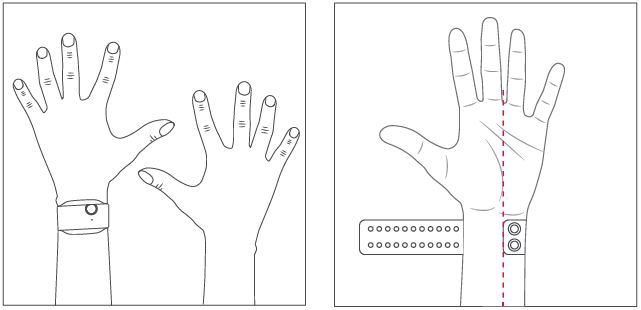
\includegraphics[width=0.33\textwidth]{../images/E4wearing.JPG}
%	\caption{A figure depicting the intended way the E4 wristband should be worn.}
%	\label{e4wearing}
%\end{figure}